
\subsection{Tiesinės nelygybės}
\begin{align*}
    \begin{aligned}
        ax + b > 0&\quad\Rightarrow\quad ax > -b     \\
        \jei a < 0&,\quad x < - b : a \quad !        \\
        \jei a > 0&,\quad x > - b : a                \\
    \end{aligned}
\end{align*}
\begin{align*}
    \begin{aligned}
        \begin{cases*} x > 1, \\ x \le 4 \end{cases*} \\
        x \in (1, 4]
    \end{aligned}
    \qquad\quad
    \begin{aligned}
        \begin{cases*} x < 1, \\ x \ge 4 \end{cases*} \\
        x \in \emptyset
    \end{aligned}
    \qquad\quad
    \begin{aligned}
        x& < 1,  \\
        x& \ge 4 \\
        x& \in (-\infty; 1)\cup[4, +\infty)
    \end{aligned}
\end{align*}

\begin{align*}
    \begin{aligned}
        11 &< 3x + 5 < 23 \  /-5   \\
        6  &< 3x     < 18 \  /: 3      \\
        2  &<  x     < 6  
    \end{aligned}
    \qquad\quad
    \begin{aligned}
        6 &< -3x < 18 \  /: 3     \\
        2 &<  -x < 6  \  /: (-1)  \\
        -6 &>  x > -2  \quad !
    \end{aligned}
\end{align*}
\textit{Dėl paskutinio pav. galima įsitikinti naudojant: }
$\begin{cases*}
    2 < -x \\
    -x < 6
\end{cases*}$

\subsection{Kvadratinės nelygybės} 

\begin{equation}
    ax^2 + bx + c \lessgtr 0
\end{equation} 

Pirmiausia suskaičiuokite x reikšmės, kuriose funkcija kerta X ašį. Prisilyginant kvadratinę nelygybę nuliui. \\
\begin{equation}
    ax^2 + bx + c = 0 \\
    D = b^2 - 4ac \\
    x_{1, 2} = \frac{-b \pm \sqrt{D}}{2a} 
\end{equation} 
\\
Kai turite X ašies kirtimo x koordinates yra du būdai spręsti toliau.
\\
Pirmasis, algebrinis, kaip suprantu, reikalauja nuliui prilygintą formulę išskaidyti į $(x \pm c)(x \pm c)$, tada vėl įvesti nelygybę ir parašyti iš formules dvi lygtis su skirtingais nelygybės ženklais. 
\begin{align*}
    \begin{aligned}
    x^2 - 60 &\ge 4 \\
    x^2 - 64 &\ge 0
    \end{aligned} \quad
    \begin{aligned}
    x^2 - 64  = 0 \\
    x^2 - 8^2 = 0
    \end{aligned}  \quad
    \begin{aligned}
    (x - 8)(x + 8) = 0 \\
    (x - 8)(x + 8) \ge 0
    \end{aligned}  \quad
    \begin{cases}
        x - 8 \ge 0 \\
        x + 8 \ge 0
    \end{cases}
    \begin{cases}
        x - 8 \le 0 \\
        x + 8 \le 0
    \end{cases}
\end{align*}
\begin{equation*}
    x \in ( -\infty; -8\,] \cup [\,8; +\infty )
\end{equation*}
\\ 
Antrajam budui reikia nusipiešti vieną tokių grafikų:

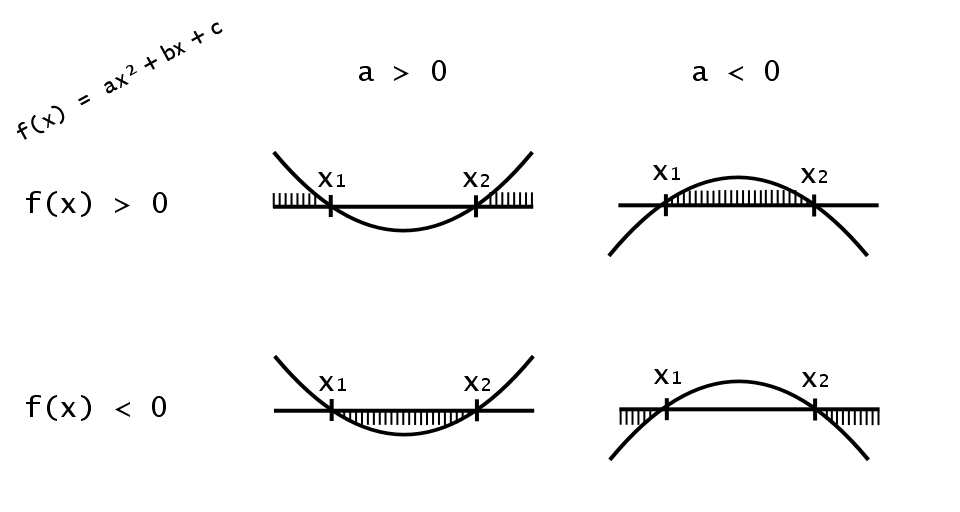
\includegraphics[max width=\textwidth]{inequalities_parabola.png}
\\
Atsakimas bus jūsų grafike užbrūkšniuota dalis.
\\
Beje, jei parabolė nekerta x ašies, x gali priklausėti, arba $(-\infty, +\infty)$, arba $\phi$. Kuris iš tų teisingas galima išsiaiškinti visu tuzinu būdų, pvz: jei, ir $a > 0$, ir $f(x) > 0$ arba, ir $a < 0$, ir $f(x) < 0$ tai x priklausys visoms realiųjų skaičių reikšmėms.


\subsection{Trupmeninės nelygybės}
% TODO: Not done yet, there's also stuff similar to critical point stuff (f(x) > 0)

\begin{equation}
    \frac{ax + b}{cx + d} \lessgtr 0, c \neq 0
\end{equation}

\begin{equation}
    \frac{f(x)}{g(x)} > 0, \jei 
    \begin{cases}
        f(x) > 0, \\
        g(x) > 0
    \end{cases} arba \quad
    \begin{cases}
        f(x) < 0, \\
        g(x) < 0
    \end{cases}
\end{equation}
\begin{equation}
    \frac{f(x)}{g(x)} < 0, \jei 
    \begin{cases}
        f(x) > 0, \\
        g(x) < 0
    \end{cases} arba \quad
    \begin{cases}
        f(x) < 0, \\
        g(x) > 0
    \end{cases} 
\end{equation}

\subsection{Rodiklinės nelygybės}

\begin{equation}
    a^{f(x)} > a^{g(x)}
\end{equation}

\begin{align}
    a > 1 \Rightarrow f(x) > g(x), \\
    0 < a < 1 \Rightarrow f(x) < g(x),
\end{align}

\begin{equation}
    \sqrt{2^{3x}} < \frac{1}{8} \quad\Rightarrow\quad
    2^{\frac{3}{2}x} < 2^{-3} \quad\Rightarrow\quad
    \frac{3}{2}x < -3 \quad\Rightarrow\quad
    x < -2
\end{equation}

\begin{equation}
    \sqrt{{(\frac{1}{2})}^{3x}} < \frac{1}{8} \quad\Rightarrow\quad
    {(\frac{1}{2})}^{\frac{3}{2}x} < {(\frac{1}{2})}^{3} \quad\Rightarrow\quad
    \frac{3}{2}x > 3 \quad\Rightarrow\quad
    x > 2
\end{equation}

\subsection{Logaritminės nelygybės}

\begin{equation}
    \log_a f(x) > \log_a g(x), \qquad a > 0, a \ne 1, b > 0
\end{equation}

\begin{equation}
    a > 1 \Rightarrow 
    \begin{cases}
        f(x) > 0, \\
        g(x) > 0, \\
        f(x) > g(x)
    \end{cases} \\
    0 < a < 1 \Rightarrow 
    \begin{cases}
        f(x) > 0, \\
        g(x) > 0, \\
        f(x) < g(x)
    \end{cases}  
\end{equation}

\subsection{Modulinės nelygybės}
\begin{center}
    $
    \begin{array}{ l | l l }
              & |f(x)| < a    \qquad & |f(x)| > a               \\
        \hline                                                  
        a = 0 & x \in \phi    \qquad & x \in \mathbb{R}         \\
        a < 0 & x \in \phi    \qquad & f(x) < -a \arba f(x) > a \\
        a > 0 & -a < f(x) < a \qquad & x \in \mathbb{R}         \\
    \end{array}
    $
\end{center}

Beje, $\sqrt{a^2} = |a| \ne {(\sqrt{a})}^2$ \\

$\sqrt{(-4)^2} \ne {(\sqrt{-4})}^2$

$\sqrt{(-4)^2} = \sqrt{16} = 4$

${(\sqrt{-4})}^2 = \phi \arba {(\sqrt{-4})}^2 = {(\sqrt{4 * -1})}^2 = {(2\sqrt{-1})}^2 = (2i)^2 = 4 * i^2 = 4 * -1 = -4$


\subsection{Trigonometrinės nelygybės}

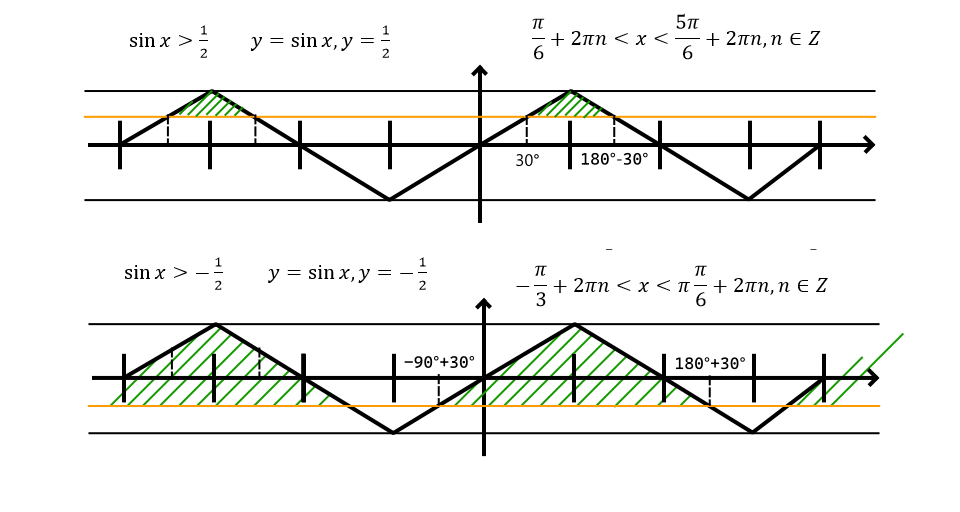
\includegraphics[max width=\textwidth]{inequalities_sin.png}
